% title: 向量与线性组合
% nav_title: 01-向量与线性组合
% date: 2026-06-07
% summary: 一个示例性的线性代数内容页，用来展示根目录内容文件夹的新组织方式，以及 LaTeX 到 HTML 的渲染效果。
% tags: 线性代数, 向量空间, LaTeX

\section{线性组合的基本想法}

在线性代数里，我们经常希望用少量基础向量去描述更多的向量。最基本的形式就是线性组合：

\[
\mathbf{v} = a_1\mathbf{u}_1 + a_2\mathbf{u}_2 + \cdots + a_n\mathbf{u}_n.
\]

这意味着，只要给定若干向量 $\mathbf{u}_1,\dots,\mathbf{u}_n$，以及一组标量 $a_1,\dots,a_n$，就可以得到新的向量 $\mathbf{v}$。

\subsection{二维情形的直观理解}

在二维平面里，若
\[
\mathbf{u}_1 =
\begin{pmatrix}
1\\
0
\end{pmatrix},
\qquad
\mathbf{u}_2 =
\begin{pmatrix}
0\\
1
\end{pmatrix},
\]
那么任意向量
\[
\mathbf{v} =
\begin{pmatrix}
x\\
y
\end{pmatrix}
\]
都可以写成
\[
\mathbf{v} = x\mathbf{u}_1 + y\mathbf{u}_2.
\]

\begin{figure}
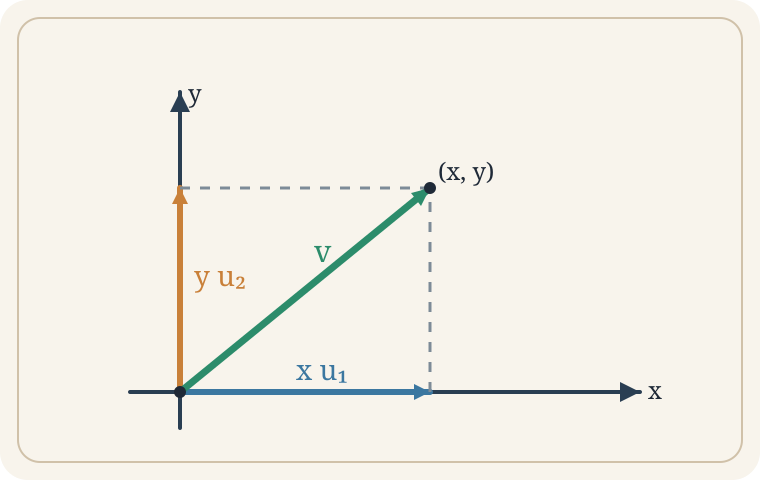
\includegraphics[width=0.74\textwidth]{assets/linear-combination.svg}
\caption{二维平面中，向量 $\mathbf{v}$ 可以看成基向量线性组合的结果。}
\end{figure}

\subsection{张成与向量空间}

\begin{definition}
给定向量组 $\mathbf{u}_1,\dots,\mathbf{u}_n$，所有形如
\[
a_1\mathbf{u}_1 + \cdots + a_n\mathbf{u}_n
\]
的向量所构成的集合，称为这组向量的\textbf{张成集}。
\end{definition}

如果一组向量能够张成整个空间，我们就说它们足以描述这个空间中的所有向量。在线性代数课程里，这会进一步引出“基”“维数”“线性无关”等核心概念。

\subsection{一个常见结论}

\begin{theorem}
在 $\mathbb{R}^2$ 中，只要两个向量线性无关，它们就能够张成整个 $\mathbb{R}^2$。
\end{theorem}

\begin{proof}
若两个向量线性无关，则它们不共线，因此它们确定了平面中的两个独立方向。任意平面向量都可以唯一地沿这两个方向分解，所以整个 $\mathbb{R}^2$ 都能写成这两个向量的线性组合。
\end{proof}

\subsection{为什么这个示例有意义}

\begin{example}
这个文件被直接放在仓库根目录下的 `A01-线性代数` 文件夹中，因此别人打开 GitHub 仓库首页后，能够立刻定位到“线性代数”这一专题，而不用先进入统一的内容总目录。
\end{example}

这正是这次结构调整的主要目标：让内容文件夹本身就成为仓库首页最直观的导航入口。
